\documentclass[12pt]{report}
%\documentclass[twoside, openright, 12pt]{report}
 
\usepackage[top=2cm, bottom=2cm, left=2cm, right=2cm]{geometry} % definition des marges

\usepackage[applemac]{inputenc}
\usepackage[T1]{fontenc}
\usepackage[francais]{babel} 
\usepackage{url}
\usepackage{graphicx}
\usepackage{titlepic}
\usepackage{titlesec, blindtext, color}
\usepackage{amsmath}
\usepackage{amssymb}
\usepackage{mathrsfs}
\usepackage{listings}
\usepackage{multirow}
\usepackage{caption}
\usepackage{minitoc}
\usepackage{perpage}
\usepackage{setspace}
\setstretch{1.5} % interligne de 1.5

%paragraph options
\setlength{\parindent}{15pt}
\setlength{\parskip}{6pt}

% enleve la mention chapitre
\titleformat{\chapter}[hang]{\bf\huge}{\thechapter}{2pc}{}

% Ligne orpheline ou veuve
\widowpenalty=10000 % empeche au maximum la coupure avant la derniere ligne 
\clubpenalty=10000 % empeche au maximum la coupure apres la premiere ligne 
\raggedbottom

\lstset{language=C, basicstyle=\scriptsize, numbers=left, numberstyle=\footnotesize, numbersep=7pt} 

\def\maketitle{
\thispagestyle{empty}

  \vspace*{6cm}
  
  \begin{center}\leavevmode
  \Large  \textbf{Structure de donn�e} \\
  \Huge Compte rendu TP1 \\
   \rule{11cm}{1pt} \\
   \normalsize Lelong G�rald  \\
    Martignoni No�l  \\
  \end{center}
      
  \cleardoublepage
  }  

% Le document --------------------------------------------------------------------------------------------------------
\begin{document}

\maketitle

\tableofcontents

\chapter{Pr�sentation du TP}

\section{Description}

L'objectif de ce TP et de cr�er une structure de donn�e du type liste chain�e � deux niveaux, ainsi que de programmer une s�rie d'algorithme pour modifier cette structure.

\section{Sch�ma de la structure de donn�es}

Les donn�es sont compos�es par une liste chain�e principale, qui contient un pointeur sur une sous liste (fig. \ref{fig:listechaineexample} p. \pageref{fig:listechaineexample}).
\begin{itemize}
\item La liste principale contient l'ann�e, la semaine, un pointeur sur une sous liste et un pointeur sur l'�l�ment suivant.
\item La sous-liste contient le jour, l'heure, l'�v�nement ainsi qu'un pointeur sur l'�l�ment suivant.
\end{itemize}

\begin{figure}[position]
   \begin{center}
   \caption{\label{fig:listechaineexample} Liste chainee}
   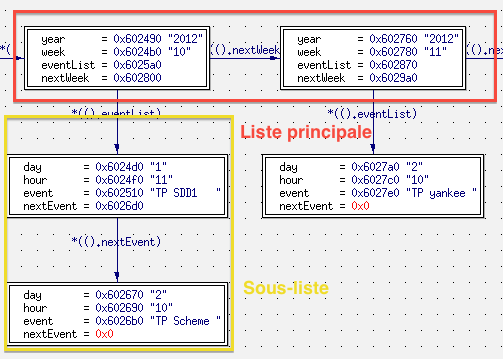
\includegraphics[scale=0.8]{listechaineeexample.png}
   \end{center}
\end{figure}

\section{Organisation du code source}

\begin{description}
\item[main.c] Programme principal
\item[struct.h] Contient les structures et �num�rations utilis�es pour d�finir un \textit{calendar}.
\item[calendar.h .c] Contient les fonctions de manipulation de \textit{calendar} de bas niveau.
\item[handler.h .c] Contient les fonctions de manipulation de \textit{calendar} de haut niveau.
\item[tools.h .c] Contient des fonctions de bas niveau sans lien direct avec les \textit{calendar}.
\end{description}

\chapter{Programme C}

\section{main.c}

\lstinputlisting[language=C]{../main.c}

\section{struct.h}

\lstinputlisting[language=C]{../struct.h}

\section{calendar.h}

\lstinputlisting[language=C]{../calendar.h}

\section{calendar.c}

\lstinputlisting[language=C]{../calendar.c}

\section{handler.h}

\lstinputlisting[language=C]{../handler.h}

\section{handler.c}

\lstinputlisting[language=C]{../handler.c}

\section{tools.h}

\lstinputlisting[language=C]{../tools.h}

\section{tools.c}

\lstinputlisting[language=C]{../tools.c}

\chapter{Compilation et tests}

\section{Makefile}

\lstinputlisting[language=make]{../makefile}

\section{Jeux de test}

\subsection{Insertion �l�ment}

\subsection{Insertion �l�ment dans liste vide}

\subsection{Suppression d'un �l�ment}

\subsection{Suppression d'un �l�ment qui n'est pas dans la liste}

\subsection{Suppression d'un �l�ment dans liste vide}

\subsection{Liste bilat�re}

\begin{figure}[position]
   \begin{center}
   \caption{\label{listechaine} Liste chainee}
   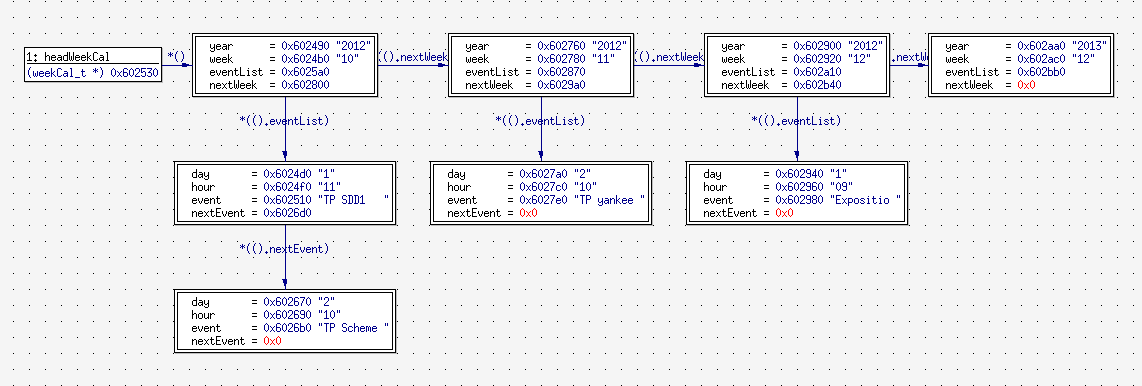
\includegraphics[scale=0.4]{listechainee.png}
   \end{center}
\end{figure}

\begin{figure}[position]
   \begin{center}
   \caption{\label{listebil} Liste bilatere}
   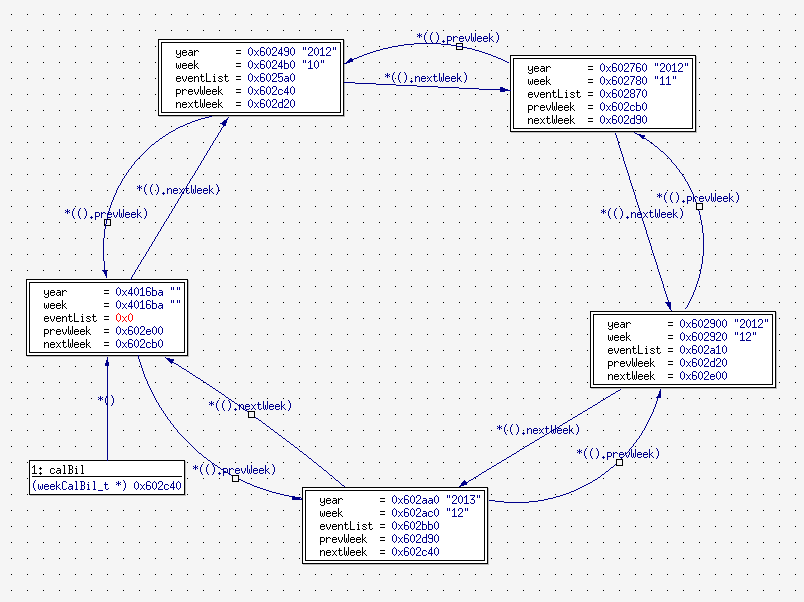
\includegraphics[scale=0.6]{listebil.png}
   \end{center}
\end{figure}


\end{document}






















